\epigraph{\textit{To them, I said, 
the truth would be literally nothing 
but the shadows of the images.... \\ Plato, The Republic (Book VII)}}  

\section{Large $N$ limit of gauge theories}

The theory of strong interactions has a gauge group SU(3). In the quest to analytically solve QCD 
`t Hooft introduced \cite{Hooft:1974aa, SCA} the idea of large $N$ limit of gauge theories by considering $SU(N)$ gauge group. 
We often associate more variables with greater complexity. But this is not always true. 
There are many class of theories which simplify in the large $N$ limit. 
This occurs because the fields are related by a certain
symmetry because of which the collective behaviour of the fields becomes more constraining 
as their number increases. This  is in some sense similar to the classical limit. The resulting
coupled degrees of freedom typically look different from the Lagrangian of the initial theory. 
It was soon after realized that the large $N$ limit of gauge theories is also related to string theory 
because roughly speaking in large $N$ limit one sums over surfaces of different genus and in string theory one sums over different world-sheets topologies. 
The idea of large $N$ has been a very fruitful area of research for decades now. 
Some developments include Migdal factorization equations, large $N$ phase transitions, 
Eguchi-Kawai (EK) volume reductions, holography, and AdS/CFT correspondence. 
The EK model ~\cite{Eguchi:1982nm} was proposed on the basis of large $N$ factorization of Wilson loops
based on the analysis of Migdal-Makeenko ~\cite{Makeenko:1979pb} \cite{Makeenko:1980vm} 
loop equations (the Schwinger-Dyson equations for Wilson loop
correlation functions) and assuming that the center symmetry was unbroken. 

In QCD, one might think that the expansion parameter is $g_{YM}$, but this is not true in the light of the 
renormalization group equations. QCD has no obvious free parameter and this makes things very difficult to calculate in 
perturbation theory. ~`t Hooft suggested to take $N$, the number of colors as a parameter. 
The large $N$ limit exists for vector as well as matrix models. QCD is an example of matrix model because the fields are 
$N \times N$ matrix (like $A_{\mu}^{ij}$) which has $N^2$ components. Since the matrix must be traceless, it should have one 
less component, but the difference is not important in the large $N$ limit. 
The vector models for example only have $N$ components. We will not discuss the large $N$ limit of vector models in this chapter. They are different from 
matrix models in following ways:

\vspace{5mm}

\begin{itemize}
\item They are sometimes soluble in large $N$ limit. 
\item Their free energy F $\sim N$ rather than $\sim N^2$ as for matrix gauge theories (admittedly this counting 
may fail for example when the theory is in a confining phase. We assume the theory is not in a confining phase for now.)
\item Their gauge coupling $g \sim 1/N$ rather than $g \sim 1/\sqrt{N}$
\item They don't have any relation to strings. 
\item Because of their different scaling, the only interactions in the standard large N vector model are ~`cactus' diagrams. 
This means that except some self energy corrections the theory is essentially free. 
\end{itemize} 

In order to better understand how we can think of large $N$ limit of QCD, it is useful to look at the QCD $\beta$-function. 
One can then check whether this limit captures the defining property of QCD - negative $\beta$ function. The perturbative 
two-loop $\beta$-function given by, 
\beq
\label{eq:beta0}
\mu \frac{dg}{d\mu} = - \frac{1}{4\pi^2} \left (\frac{11N - 2n_{f}}{3} \right)g^3  - \frac{1}{4\pi^4} \left (\frac{34N^3 - 13 N^{2} n_{f} + 3nf}{3N}\right)g^5 + \mathscr{O}(g^7)
\eeq

This has clearly no sensible large $N$ limit. But we can make an interesting observation. The LHS of (\ref{eq:beta0}) goes as 
$ \sim g$, whereas RHS $ \sim g^3 N$. `t Hooft considered the limit where $N \to \infty$ and $g^2 \to 0$ while $\lambda = g^2 N $ 
remains fixed. $\lam$ is the `t Hooft coupling. In this limit, we get, 

\beq
  \label{eq:beta1}
\mu \frac{d\lambda}{d\mu} = - \frac{11}{24 \pi^2} \lambda^2 -  \frac{17}{192 \pi^4} \lam^3 + \mathscr{O}(\lambda^4) 
\eeq

As can be readily seen, perturbation theory predicts that the `t Hooft limit of QCD is an asymptotically free
theory. So, that is a good first step. It is also natural to assume that the $\Lambda_{\text{QCD}}$, 
the scale parameter of strong interactions is held fixed as $N \to \infty$. One important feature of ~\ref{eq:beta1} 
is that it is independent of number of flavors, $n_{f}$. The 
number of quark degrees of freedom is $\mathscr{O}$(N) in the
`t Hooft limit, and hence sub-leading with respect to the number of gluon degrees of freedom, which is $\mathscr{O}$ $(N^{2})$. 
To get an idea of large $N$ limit, consider the following Lagrangian, 

\begin{equation}
L = \frac{1}{g} \mathrm{Tr} \Bigg( (\partial \Phi)^2 + \Phi^2 + \Phi^3 + \Phi^4  \Bigg) 
\end{equation} 

We can rescale $ \Phi = g \tilde{\Phi}$  to get, 

\begin{equation}
L = \mathrm{Tr} \Bigg( (\partial \tilde{\Phi})^2 + \Phi^2 + g \tilde{\Phi}^3 + g \tilde{\Phi}^4  \Bigg)
\end{equation} 

The big field $\Phi$ which we think of as potentially including scalars $\phi$, gauge fields $A_{\mu}$, and fermions $\Psi_{a}$  all of which are N $\times$ N matrices.

So, the propagator $\langle \Phi \Phi \rangle$ goes as $g^2$ i.e $\lambda/N$. In a generic matrix theory there will be three point and four-point Fig.(\ref{fig:dl2}) interaction
vertices. Both types of vertices come with the same factor of $N/\lambda$


Let's consider the Lagrangian (actually, a modified version of Yang-Mills Lagrangian, and also incomplete)
\begin{equation}
  \label{eq:action1}
  \mathscr{L} \sim  \frac{1}{g^2} \left [ -\frac{1}{4} F_{\mu\nu b}^{a}F^{\mu\nu b}_{a} + \text{fermions} \right]  ,
\end{equation}
with $F_{\mu\nu b}^{a} = \partial_{\mu} A^{a}_{\nu b} - \partial_{\nu} A^{a}_{\mu b} + i [A_{\mu}, A_{\nu}]^{a}_{b}$. 

The `t Hooft limit is the limit where $N \to \infty$ and $g_{\text{YM}} \to 0$ while $\lambda = g_{\text{YM}} N $ remains fixed. $\lam$ is the 
`t Hooft coupling. Also, the advantage of using this particular form of the Lagrangian is that any vertex has the same factor $g_{\text{YM}}$. 
We need not worry about the difference between three-gluon, four-gluon vertex contributing to different factors. So, both diagrams in Fig.(\ref{fig:dl2})
contribute the same $N/\lambda$. 


\begin{figure}
\begin{center}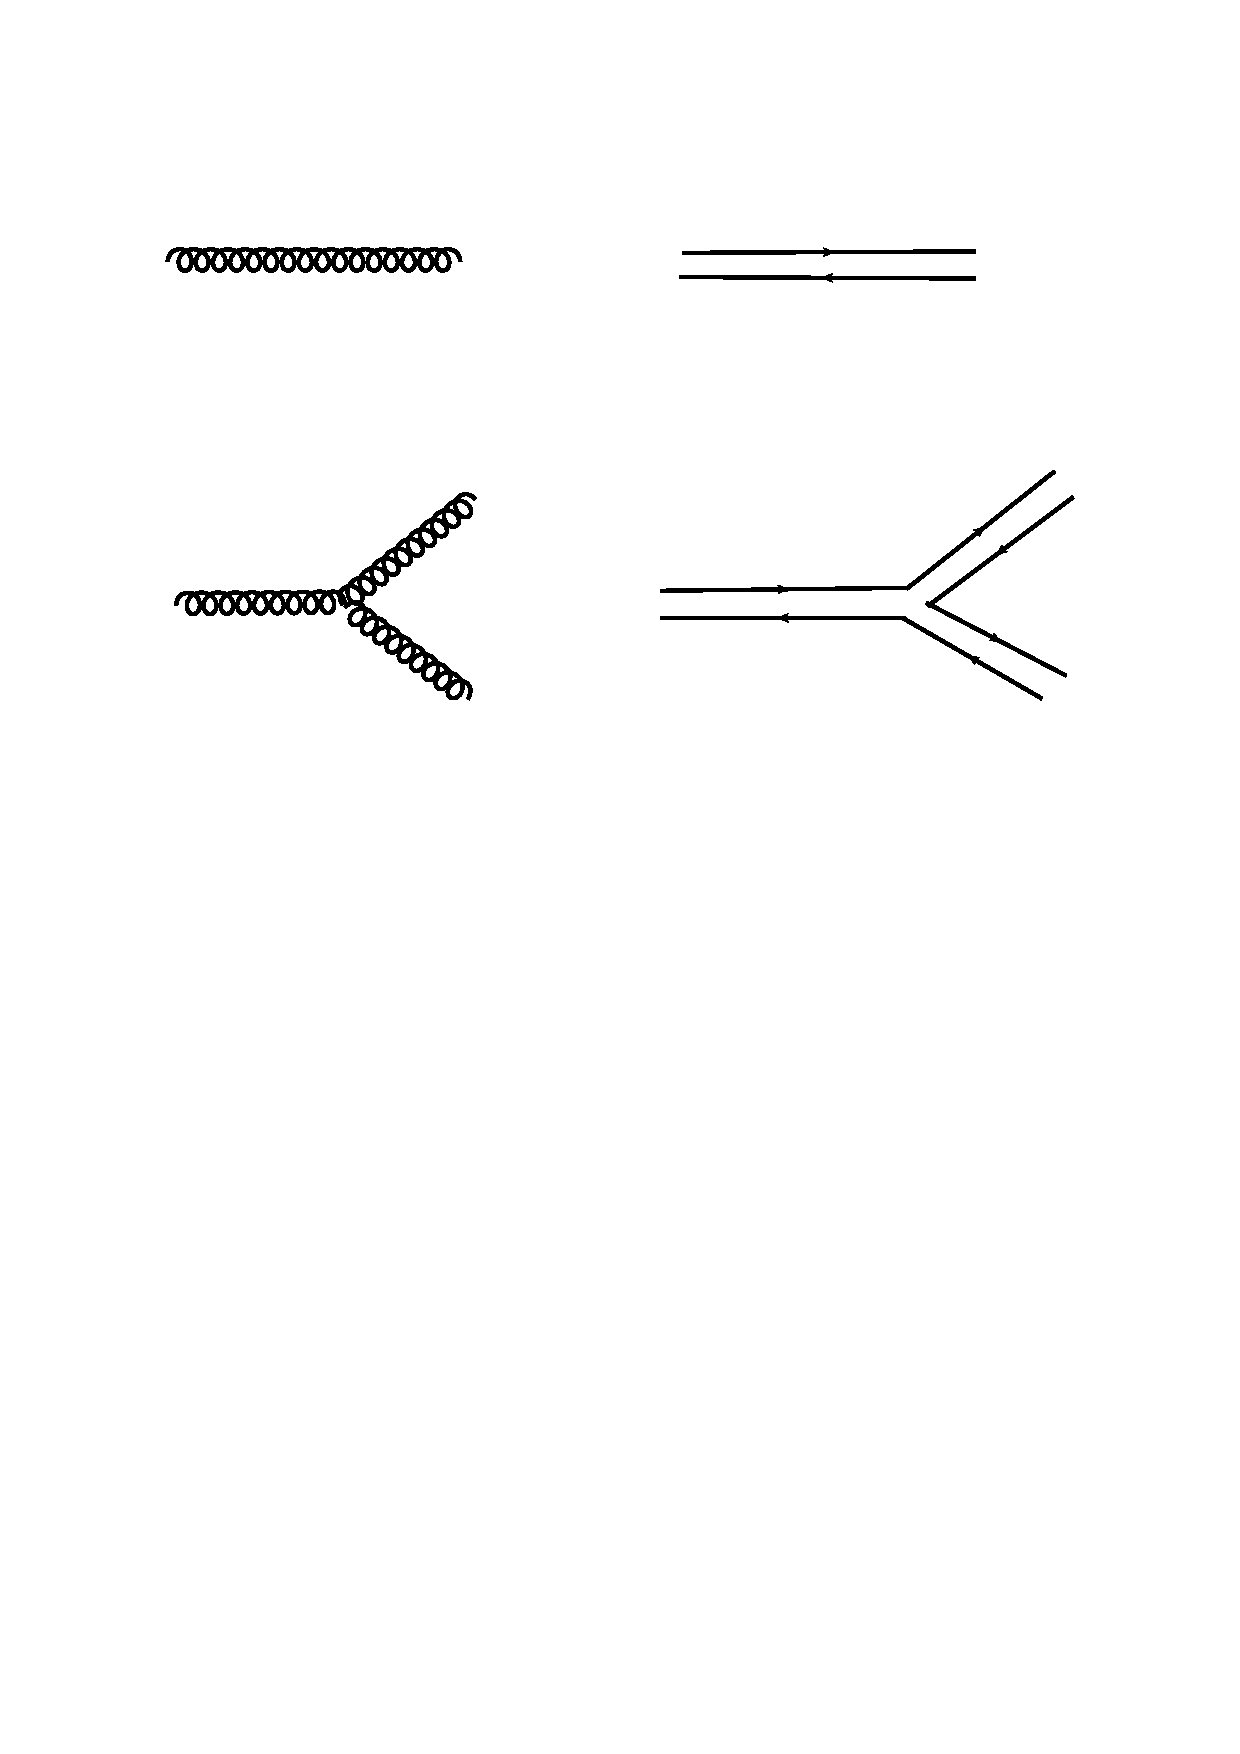
\includegraphics[width=0.35\textwidth]{./Figures/DL1}\end{center}
%\caption{\label{fig:dl2}Both diagrams contribute $\sim N/\lambda$. Note that E = F = 0 and V = 1 for both. }
\end{figure}


\begin{figure}
\begin{center}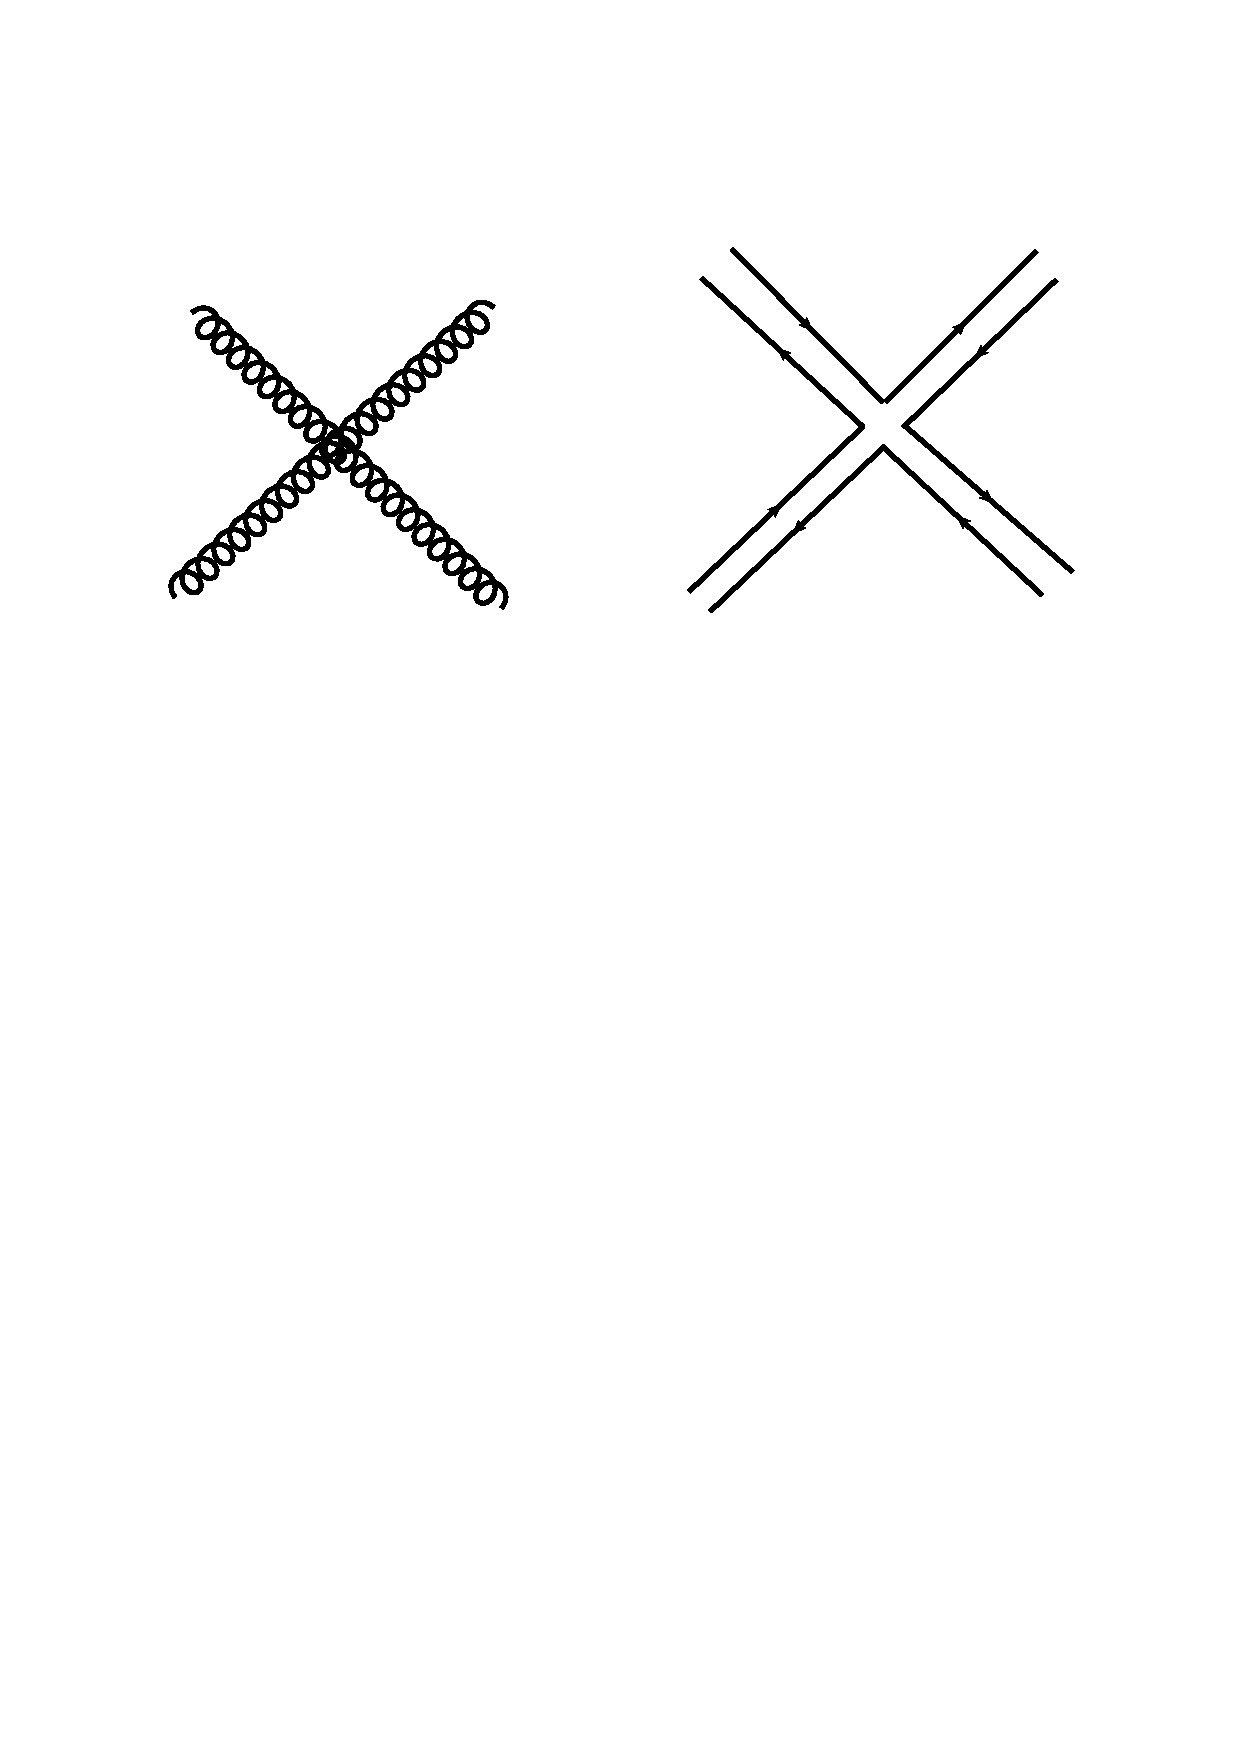
\includegraphics[width=0.35\textwidth]{./Figures/DL3}\end{center}
\caption{\label{fig:dl2}All the diagrams above contribute $\sim N/\lambda$.}
\end{figure}

With our current normalization 
\footnote{We should be careful about field normalizations when doing large N counting for correlation functions. } 
the propagator $\langle \Phi \Phi \rangle$ goes like $\lambda/N$. The propagator in the double line notation appears in Fig.(\ref{fig:dl2}). 
We can naively see that the gluon propagator and quark propagator $ \sim 1/N$ 
whereas, the vertex $ \sim N$ in the `t Hooft limit. 

We can write the gluon propagator as (shown in Fig.(\ref{fig:dl2})), 

\begin{equation}
  \label{eq:gluon}
   A^{a}_{\mu b}(x) A^{c}_{\nu d}(y) = \left ( \delta^{a}_{d}\delta^{c}_{b} - \frac{1}{N} \delta^{a}_{b}\delta^{c}_{d}\right)
   \mathscr{D}_{\mu\nu}(x-y) , 
\end{equation}

In some sense, the gauge field is represented by a ``quark" with index $i$, and an ``antiquark" with index $j$. 
The second term in the parentheses is because we need to make the gluon field traceless for SU($N$) group we are
considering. It would not be present if we were working with U($N$). In any case, in the large $N$ , the distinction is unimportant.  
Following the gluon line indices we see, the index pair at the beginning is the same as that at the end. In some sense, 
a gluon propagates like quark--anti-quark pair. This observation was made by `t Hooft when he devised the double-line 
notation. Loosely speaking, we will draw as many lines in a propagator as the indices it carries. Therefore, quark propagator 
is denoted by a single line since it carries one index, whereas a gluon propagator is drawn using double lines, see Fig.(\ref{fig:dl2})
For SO($N$) or USp($N$) theories, the adjoint representation may be written as a product of two fundamental representations 
rather than a product of a fundamental and an anti-fundamental representation (like done for SU($N$) and U($N$)). Since the
fundamental representation is real, there are no arrows on the propagators \footnote{Recall that arrows fix the orientation of complex fields}. 
Generally, a vacuum diagram has the following dependence on $g_{\text{YM}}$ and $N$, 

\[  \text{Amplitude} \sim \text{diagram} \sim (g_{\text{YM}})^{E} (g_{\text{YM}})^{-V} N^{F} \] 
where E is the number of propagators, V is the number of vertices, F is the number of faces. This has no sensible
$N \to \infty$ limit, since there is no upper limit on F. However, `t Hooft suggested that we can
take the limit $N \to \infty$ and $g_{\text{YM}} \to 0$ but keep $\lambda = g_{\text{YM}} N $ remains fixed. 
\[ \text{diagram}(V,E,F) \sim N^{V-E+F} \lambda^{E-V}  \sim N^{\chi} \lambda^{E-V} \] 
where, $\chi = F + V - E$ is assured by a theorem due to Euler. 

\emph{Theorem}: Given a surface composed of polygons with F faces, E edges and V vertices, the Euler character satisfy
$\chi = F + V - E = 2 - 2h$. 
here, $h$ is the number of handles (also known as `genus' ) of the surface. See Fig(3) for example. 
Since, in the large $N$ limit, the diagrams with $h = 0$ contribute most 
the large $N$ limit is also known as the planar limit (because $h=0$ means no handles like spheres). Since each Feynman 
diagram can be considered as a partition of the surface separating it into polygons, then the
above theorem also works for our counting in $N$. Only planar diagrams survive in the large $N$ limit.  

As an example, let's consider the diagram shown in Fig (\ref{fig:dia1}), which has four 3-point vertices, six propagators, and four index (color) loops. 
At this point, we can make some remarks. 1)  The sphere (or the plane) has the largest Euler characteristic, $\chi = 2$. 
Planar can be drawn on plane (without crossing), also called "non-crossing", 2) In QED, the expansion parameter is $e^2/4\pi$ = 
1/137 which implies that $ e = 0.3$. But in fact, the true expansion parameter in QED is actually  $e^2/4\pi^2$. It is little gloomy 
for Yang-Mills since there is no
extra $1/4\pi$ and the expansion parameter is $1/N$ or $1/N^2$. This argument is initially due to Witten found in 
\cite{SCA}. 


\begin{figure}
 \label{fig:dia1}
\begin{center}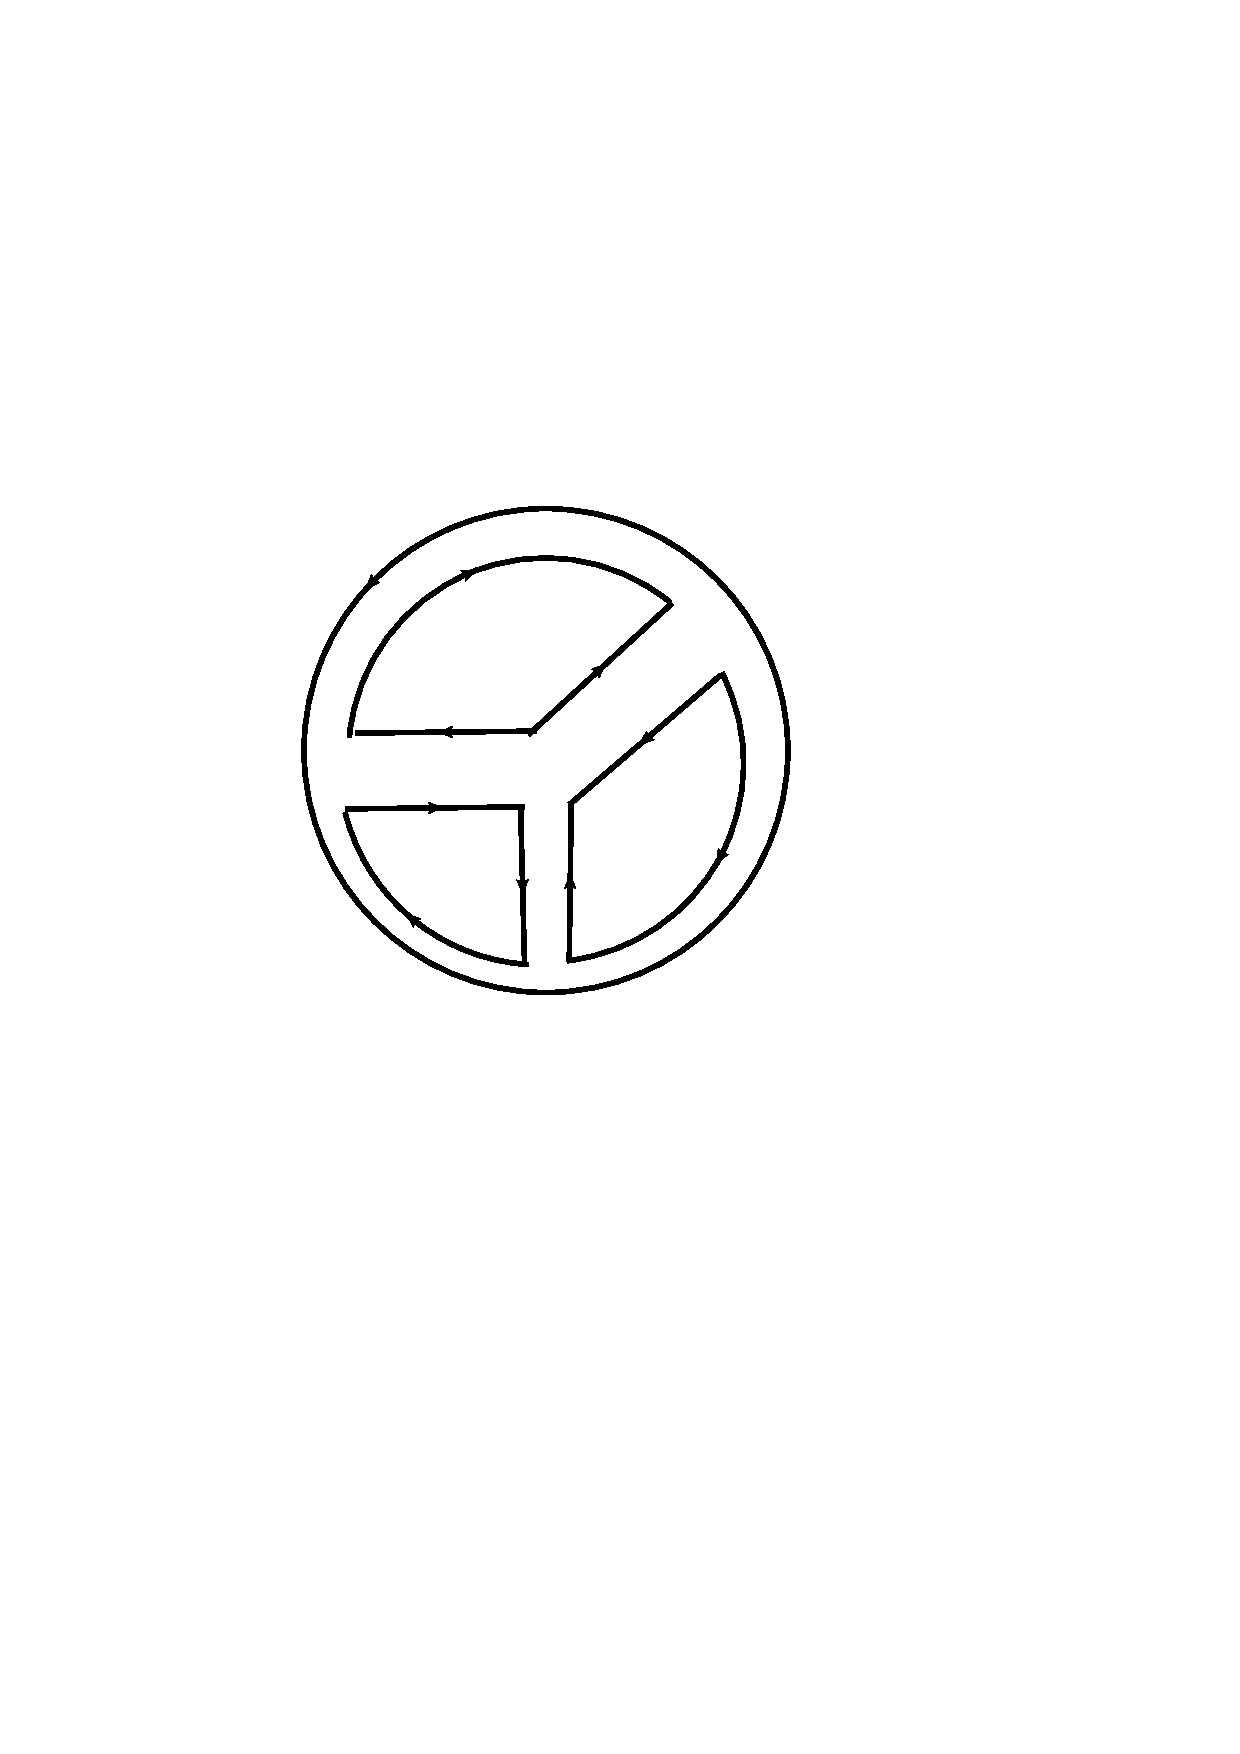
\includegraphics[width=0.25\textwidth]{./Figures/DL5}\end{center}
\caption{\label{fig:dia1}This contributes $\sim N^2 \lambda^2$.}
\end{figure}


\begin{figure}
\begin{center}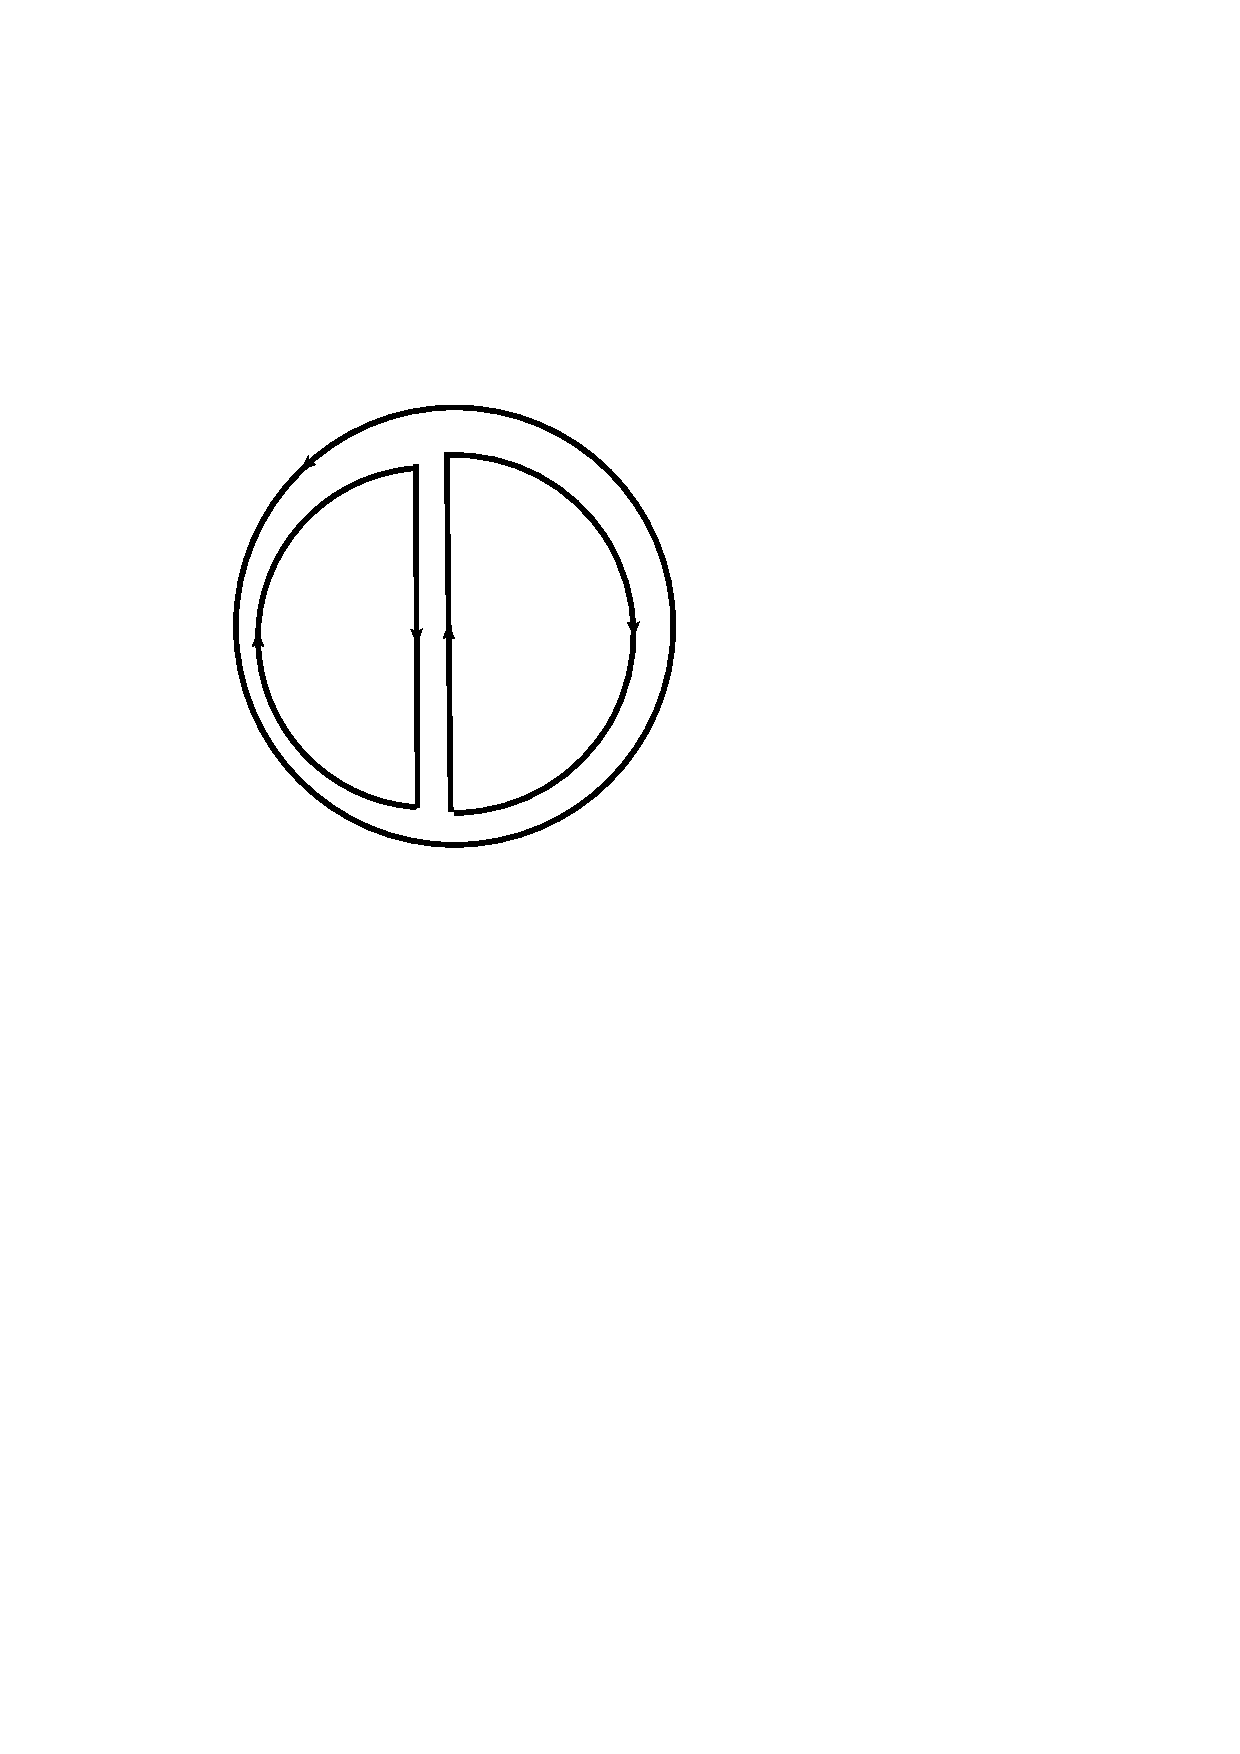
\includegraphics[width=0.25\textwidth]{./Figures/DL4}\end{center}
\caption{\label{fig:dl99}The has $E=3$, $V=2$ and $F=3$ and contributes $\sim N^2 \lambda $.}
\end{figure}
The free energy can be expressed as, 
\begin{align}
  \label{eq:logZ}
   \text{log} \mathscr{Z} =&\sum_{h=0}^{\infty} N^{2-2h} f_{h}(\lambda) \\ 
   				    =& N^{2} f_{0}(\lambda) + f_{1}(\lambda) + \frac{1}{N^2} f_{2}(\lambda) + \cdots
\end{align}
The first term comes from the planar diagrams, the second term from the genus-1 diagrams, and so on.
Hence, in the large $N$ limit, the free energy goes as $\mathscr{O}(N^2)$. 
One might think that the free energy diverges in the large $N$ limit, but we actually calculate, 

\[ \displaystyle\lim_{N \to \infty} \frac{F}{N^2} = \cdots  \] 
which has a sensible large $N$ limit. 

\subsection{Factorization and master field in the planar limit}
General observables we consider are correlation functions of gauge invariant operators, 
\beq
 \label{eq:gsop}
\langle \mathcal{O}_{1}(x_{1}) \mathcal{O}_{2}(x_{2}) \cdots \mathcal{O}_{n}(x_{n})\rangle_{\text{con}}
\eeq 
we will assume that $\mathcal{O}$ is a single trace operator. it is enough to just consider them since the multiple trace operator are just products of them. 
\begin{itemize}
\item Single-trace operators : $\mathrm{Tr}(F_{\mu\nu}F^{\mu\nu}) , \mathrm{Tr}(\Phi^n)$ 
\item Double-trace operators : $\mathrm{Tr}(F_{\mu\nu}F^{\mu\nu})\mathrm{Tr}(\Phi^2)$ 
\end{itemize}
Generally, single trace operators are like, 
\begin{equation}
 \mathcal{O}(x)  = \mathrm{Tr} (\Phi_{1}(x) \cdots \Phi_{k}(x)) 
 \end{equation}
An important thing is to understand how does (\ref{eq:gsop}) behaves in the large $N$ limit. Consider the following, 


\beq
 \label{eq:trick1}
 \mathscr{Z}[J_{1}, \cdots J_{n}] = \int \mathcal{D}A \mathcal{D}\Phi \cdots \exp \left [ S_{0} + N \sum_{j} \int J_{i}(x)\mathcal{O}_{i}(x) \right] 
\eeq 
Then, (\ref{eq:gsop}) can be written as, 
\beq
 \label{eq:trick2}
\langle \mathcal{O}_{1}(x_{1}) \mathcal{O}_{2}(x_{2}) \cdots \mathcal{O}_{n}(x_{n})\rangle_{\text{con}} = 
\displaystyle\lim_{\text{all} ~ J \to 0} \frac{\delta^{n} \text{log} \mathscr{Z}}{\delta J_{1}(x_{1}) \cdots \delta J_{n}(x_{n}) } \frac{1}{N^n}
\eeq 
But, we know that 
\beq
\text{log} \mathscr{Z}[J_{1} \cdots J_{n}] = \sum_{h=0}^{\infty} N^{2-2h} f_{h}(\lambda, \cdots)
\eeq
So, we get, 
\beq
 \label{eq:trick3}
\langle \mathcal{O}_{1}(x_{1}) \mathcal{O}_{2}(x_{2}) \cdots \mathcal{O}_{n}(x_{n})\rangle_{\text{con}} \sim N^{2-n} \left [ 1 + \mathscr{O}(\frac{1}{N^2}) \right] 
\eeq 
and it is equivalent to,  
\[ \langle I \rangle \sim \mathscr{O}(N^{2}) + \mathscr{O}(N^{0}) \] 
\[ \langle \mathcal{O} \rangle \sim \mathscr{O}(N) + \mathscr{O}(N^{-1}) \] 
\[ \langle \mathcal{O}_{1}\mathcal{O}_{2}\rangle_{\text{con}} \sim \mathscr{O}(N^{0}) + \mathscr{O}(N^{-2}) \] 
\[ \langle \mathcal{O}_{1}\mathcal{O}_{2}\mathcal{O}_{3} \rangle_{\text{con}} \sim \mathscr{O}(N^{-1}) + \mathscr{O}(N^{-3}) \] 


This implies that for two gauge-invariant operators, A and B (in the large $N$ limit) 
\[ \langle AB \rangle \sim \langle A \rangle  \langle B \rangle + \mathscr{O}(\frac{1}{N^2}) \] 
The variance of operators vanish in this limit and there are no fluctuations. All this has been done for 
the case of pure gauge theory but this can be extended to fermions as well. To summarize, - the average 
value is the only calculated value via the master field, which we will now discuss. 
Another immediate consequence of this can be applied to Wilson loop as done by Migdal. 
We can show that the following has, 
a decoupling property in the large $N$ limit, 

\beq
 \label{eq:migdal1}
\langle \phi(\mathcal{C}_{1})~ \phi(\mathcal{C}_{2})\rangle \to \langle \phi(\mathcal{C}_{1})\rangle \langle \phi(\mathcal{C}_{2})\rangle
\eeq

The above equation ~\ref{eq:migdal1} implies that $ \phi(\mathcal{C})$ can be considered as a classical field in loop space, 
but it does not imply that the gauge field, $A_{\mu}$ become classical in this limit. 
As it has been discussed above, in the large $N$ limit the path-integral is peaked around a particular configuration. 
This is tied to the idea of a master field (coined by Coleman) initially due to Witten. In this limit, the probability of finding 
any gauge-invariant 
quantity away from its expectation value goes to zero as $N \to \infty$ \cite{Gopakumar:1994iq}.
The best way to think of the master field is to draw an analogy with the path-integral approach. 
It tells us that Green's functions for a quantum theory are obtained by summing over all possible classical motions. 
In the limit that $\hbar \to 0$, the measure in the functional space becomes sharply concentrated about the solution to
 the classical equations of motion, in the limit of vanishing $\hbar$, 
all quantities are given by their value evaluated at the classical solution. 
In the case of the large $N$ limit of a gauge theory, there exists a master field configuration. 
All gauge-invariant operators expectation value can be evaluated using this master field. 
In case of large $N$ QCD, the master field(s) are four $N \times N , M_{i}$ matrices, where $N \to \infty$.  
Some observations are in order now: 

\begin{itemize}
\item We can calculate all the correlation functions of the invariant observables simply by taking the trace of the product of master fields and not doing any integrals. 
\item The master field is not unique since we are interested only in gauge-invariant quantities, any gauge transform of a master field is also a master field. 
So more precisely, one should talk about ~`master orbit of the gauge group'. 
\item For the classical analogy, we have a well-defined method of finding the single field configuration, i.e by solving classical equations of motion. 
But finding the master field is not a panacea, one does not have a well-defined prescription yet.
\end{itemize} 
Even after not being able to solve say for ex: large $N$ QCD in four dimensions, this is an amazing reformulation of the problem of summing only all planar graphs. 





\section{AdS/CFT correspondence} 
The study of non-perturbative formulations of superstring theories is greatly facilitated by the idea of AdS/CFT correspondence. AdS/CFT is 
a strong/weak duality between two theories first proposed by Maldacena in 1997. 
It is inspired by the structure and symmetries of the space-time and the conformal field theory (CFT). 
This conjecture is again an example of how interesting the large $N$ limit of gauge theories can be and since we have already discussed 
that in the previous section, we can start to formally discuss the holographic conjecture (or AdS/CFT correspondence). We will first review 
some useful concepts from String theory for stating this conjecture and then discuss the decoupling limit which is central to the idea of this 
correspondence. 





\subsection{D$p$-branes, and black $p$-branes} 

The low-energy limit ($l_{s} \to 0$) of string theory describes classical gravity (called `supergravity'). 
The black $p$-branes are solutions of supergravity. They can also be thought of as black holes that extend in $p$ spatial dimensions. 
$\textit{Dp-branes}$ are extended objected in (p+1) dimensions. 
They have their own identity in string theory and are the central motivation for AdS/CFT correspondence. 
A Dp-brane is defined as a hypersurface where open strings can end with Dirichlet boundary conditions (endpoints fixed). 
The open-string picture of D-brane describes a p+1 dimensional SYM. D3-brane is special because the world volume is four dimensional 
and that is where the SYM gauge theory lives. The closed-string picture of D-branes relies on the fact that the closed strings do not have to 
be attached to the D-branes. They can propagate freely in directions orthogonal to the brane and live in extra dimensions. 
It is also important to note here that D-branes break half of the supersymmetry and are BPS states. 
The same use of $p$ for both black $p$-branes and $\textit{Dp-branes}$ is confusing. 
However, Polchinski \cite{Polchinski:1995mt} realized that stack of Dp-branes and extremal black p-branes are the same objects.
As mentioned before, D-branes give rise to gauge theories. The open string states are described with a $N \times N$ matrix. 
In the low energy approximation, this gives rise to supersymmetric Yang-Mills theory. The gauge theory is controlled by two parameters, 
$\lambda, N$, whereas, in the supergravity, we have the string length, $l_{s}$ and the string coupling ($g_{s}$). 

In general, the superstring theory contains both closed and open strings. The former mediates gravitational force, and the latter mediates the gauge interactions. 
Open strings can end in objects which are called $\textit{D-branes}$. While the closed string can propagate anywhere in the bulk (1+9)-dimensional spacetime, 
the endpoints of an open string must be attached to the $\textit{D-branes}$.  As a particular case of this $\textit{D-branes }$, we have $\textit{D-particles}$, 
which look like pointlike objects. In the low-energy limit, the strings can be viewed as particles. We can express the black hole as a combination of N $\textit{D-particles}$, 
where N, the number of $\textit{D-particles}$ is large and it implies that the geometry is weakly curved and size of black hole is large. Quantum gravity effects become
large when N is small. 



\subsection{The decoupling limit} 

The limit in which the conjecture holds can be argued as follows. Consider the gauge theory in four dimensions which are associated with the world-volume of D3 branes. 
The action for string theory with $D3$-branes can be written as, 

\begin{equation}
S = S_{\text{bulk}} + S_{\text{brane}}  + S_{\text{interaction}} 
\end{equation}

where $ S_{\text{bulk}}$ is the action of closed strings in the bulk (some six-dimensional space), 
$S_{\text{brane}}$ is the action due to open strings attached to $D3$-branes. The third term is just the interaction term between
the open and closed string pieces. It is worthwhile to note that $S_{\text{interaction}} \approx g_{s} l_{s}^4$, and vanishes
in the low-energy approximation. In such a situation, the entire action is factored into bulk and brane parts. 
The bulk parts represent the SUGRA and brane then represents $\mathcal{N}=4$ SYM. 
This is only one half of the story. Another half can be seen by looking at the extremal $p$-brane 
and noting that the low-energy limit is similar to taking the near-horizon limit and in that case the 
factorization gives us like before SUGRA in the bulk
but the other part gives the $AdS_{5} \times S_{5}$. 
Therefore, in the large $N$ limit, $\mathcal{N}=4$ SYM on $R^{3,1}$ is dual to Type IIB SUGRA on $AdS_{5} \times S_{5}$. 
The limit and the complete steps are shown in Fig.(\ref{fig:AdS1}). 

\begin{figure}[h!]
\label{fig:AdS1} 
  \centering
      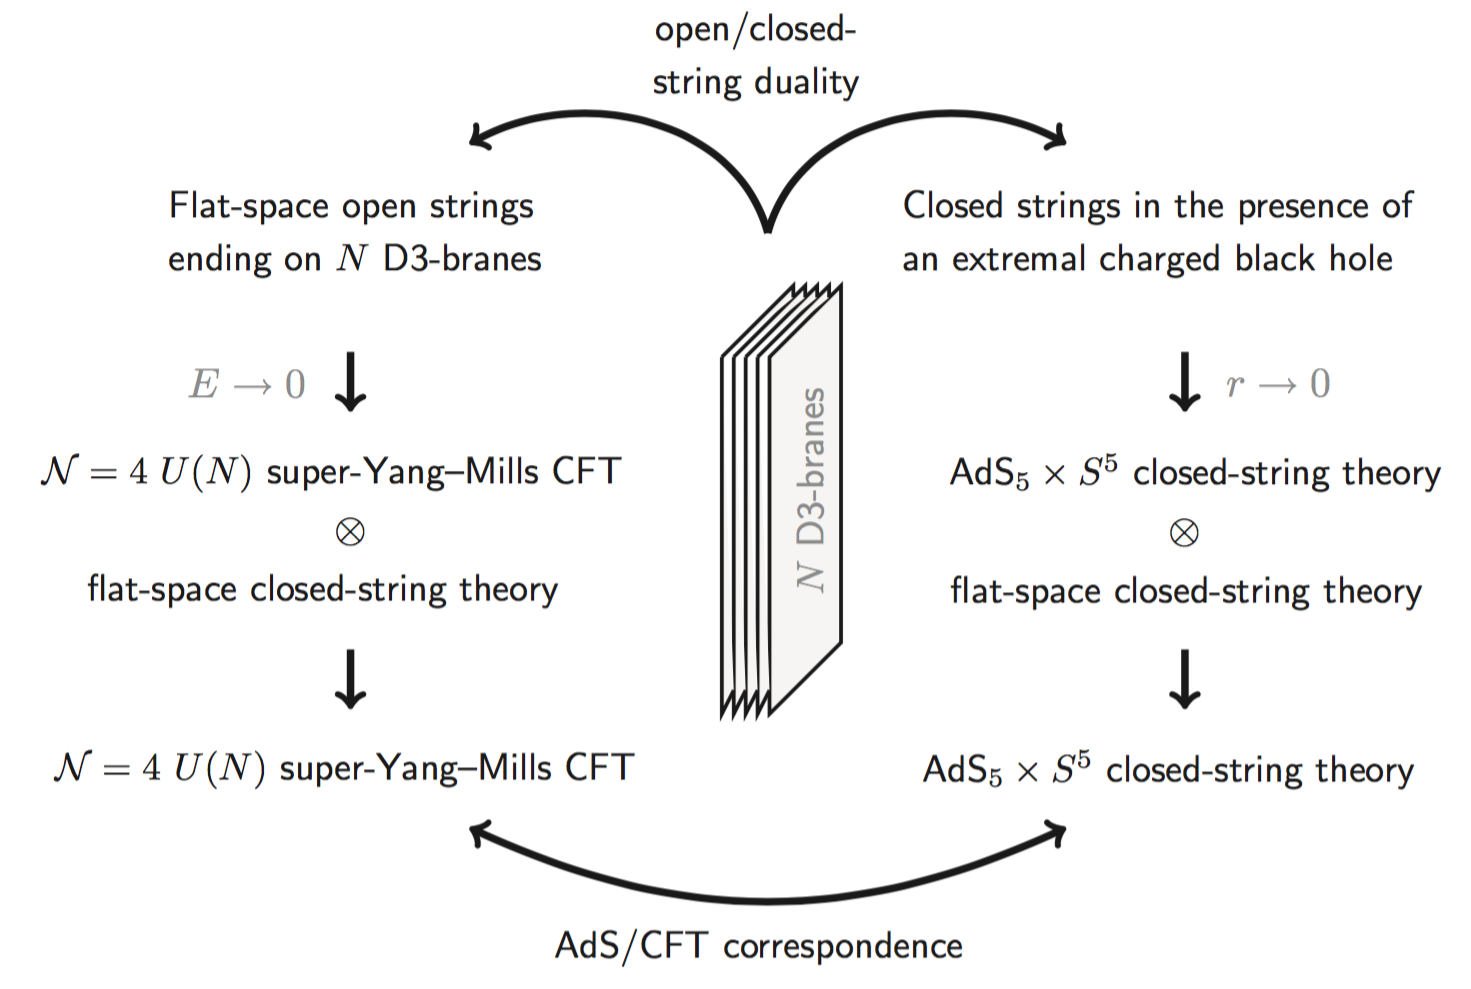
\includegraphics[width=0.9\textwidth]{./Figures/ads22.jpg}
  \caption{\label{fig:AdS1}Diagrammatic representation of the duality. Picture from \cite{ZEA}.}
\end{figure}



\subsection{Symmetries, degrees of freedom, and holographic dictionary} 

AdS/CFT correspondence can also be loosely suggested based on the following observation. First note that 
the line element of the $AdS$ space  in $(d+1)$-dimensions is given by, 
\beq
ds^2\,=\,{L^2\over z^2}\,(-dt^2+d\vec x^2+dz^2)\,\,,
\label{AdS_metric}
\eeq
The constant $L$ is a global factor in (\ref{AdS_metric}), which we will refer to as the anti-de Sitter radius. 
The (conformal) boundary of the $AdS$ space is located at $z=0$. Notice that the metric (\ref{AdS_metric}) is singular at $z=0$. 
This means that  we will have to introduce a regularization procedure in order to define quantities in the $AdS$ boundary.


The isometries of (d+1)- dimensional anti-De-Sitter space is $SO(d,2)$ symmetry which is the same as the conformal symmetry of \
$d$-dimensional Minkowski space. However, the $(d+1)$-dimensional de-Sitter space has isometry group of $SO(d+1,1)$ symmetry, 
which \textit{can be} a symmetry group of \textit{d}-dimensional Euclidean space.  In addition, we have the isometries of $S^{5}$ 
which form SU(4), which is $\approx$ SO(6). This group is same as the R-symmetry of the $\mathcal{N}$ = 4 SYM theory. The full isometry supergroup
of the $AdS^{5}$ $\times$ $S^{5}$ background is $SU(2, 2|4)$, which is identical to the $\mathcal{N}$ = 4 superconformal symmetry.

Firstly, we will discuss the QFT side. To regulate the theory we put both a UV and IR regulator. We place the system in a spatial 
box of size $R$ (which serves as an IR cutoff)  and we introduce a lattice spacing $\epsilon$ that acts as a UV regulator. In $d$ 
spacetime dimensions the system has $R^{d-1}/\epsilon^{d-1}$ cells. Let $c_{QFT}$ be the number of degrees of freedom per 
lattice site, which we will refer to as the central charge. Then, the total number of degrees of freedom of the QFT is:
\beq
N_{dof}^{QFT}= \Big({R\over \epsilon}\Big)^{d-1}\,\,c_{QFT}\,\,.
\eeq
The central charge is one of the main quantities that characterize a CFT. If the CFT is  a 
$SU(N)$ gauge field theory,  such as the theory with four supersymmetries which will be described below, the fields are $N\times N$ 
matrices in the adjoint representation which, for large $N$, contain $N^2$ independent components. Thus, in  these $SU(N)$ CFT's
 the central charge scales as  $c_{SU(N)}\sim N^2$. Central charges scale as the number of generators of a group when N is large. 
We can then compute the number of degrees of freedom of the $AdS_{d+1}$ solution. According to the holographic principle and to the 
Bekenstein-Hawking formula, the number of degrees of freedom contained in a certain region is equal to the maximum entropy and is given by
\beq
N_{dof}^{AdS}={A_{\partial}\over 4 G_N}\,\,,
\eeq
with $A_{\partial}$ being the area of the region at boundary $z\to 0$ of  $AdS_{d+1}$. Let us evaluate $A_{\partial}$ by integrating
 the volume element corresponding to the metric (\ref{AdS_metric}) at a slice $z=\epsilon\to 0$:
\beq
A_{\partial}\,=\,\int_{{\mathbb R}^{d-1},\, z=\epsilon}\,
 d^{d-1}\,x\,\sqrt{g}\,=\,\Big({L\over \epsilon}\Big)^{d-1}\,\
 \int_{{\mathbb R}^{d-1}}\, d^{d-1}\,x\,\,.
 \label{A_delta_unregularized}
 \eeq
The integral on the right-hand-side of (\ref{A_delta_unregularized}) is the
the volume of ${\mathbb R}^{d-1}$, which  is infinite. As we did on the QFT side, we regulate it by putting the system in  a box of size $R$:
\beq
\int_{{\mathbb R}^{d-1}}\, d^{d-1}\,x=R^{d-1}\,\,.
\eeq
Thus, the area of the $A_{\partial}$ is given by:
\beq
A_{\partial}\,=\,\Big({RL\over \epsilon}\Big)^{d-1}\,\,.
\eeq
Let us next  introduce the Planck length $l_P$ and the Planck mass $M_P$ for a gravity theory in $d+1$ dimensions  as:
\beq
G_N\,=\,(l_P)^{d-1}\,=\,{1\over (M_P)^{d-1}}\,\,.
\label{Planck_l_M}
\eeq
Then, the number of degrees of freedom of the $AdS_{d+1}$ space is:
\beq
N_{dof}^{AdS}={1\over 4}\, \Big({R\over \epsilon}\Big)^{d-1}\,
 \Big({L\over l_P}\Big)^{d-1}\,\,.
\eeq
By comparing $N_{dof}^{QFT}$ and $N_{dof}^{AdS}$  we conclude that they scale in the same way with the IR and UV cutoffs  $R$ and $\epsilon$ and we can identify:
\beq
{1\over 4}\,\,\, \Big({L\over l_P}\Big)^{d-1}\,=\,  c_{QFT}\,\,.
\label{holo_centralCharge}
 \eeq


The action of our gravity theory in the $AdS_{d+1}$ space of radius $L$ contains a factor $ L^{d-1}/G_N$. 
Thus, taking into account the definition of the Planck length in (\ref{Planck_l_M}), we conclude that the classical  gravity theory is reliable if:
\beq
{\rm classical\,\, gravity\,\, in\,\, AdS}\to \Big({L\over l_P}\Big)^{d-1} \gg 1\,\,,
\eeq
which happens when the $AdS$ radius is large in Planck units. Since the scalar curvature goes like $1/L^2$, the curvature 
is small in Planck units. Thus, a QFT has a classical gravity dual when $c_{QFT}$ is large, or equivalently if there is a large 
number of degrees of freedom per unit volume or a large number of species (which corresponds to large $N$ for $SU(N)$ gauge theories). 



\section{Lower dimensional SYM theories and their holographic duals}

The AdS/CFT correspondence (also gauge/gravity duality) is a conjecture which relates
the string theory or M-theory on a background of the form 
$ AdS_{d+1} \times S^{'} $, where $ AdS_{d+1}$ has an 
space-time dimension $\textit{d+1}$, and $S^{'}$ is compactified manifold 
(called ~`spheres'). The conjecture tells that this theory is dual to conformally invariant quantum field theory 
in space-time of dimension $\textit{d}$, which is, in fact, the boundary of the $AdS_{d+1}$. This conjecture can be 
viewed as a natural realization of the holographic principle, which states that all of the information inside a black hole should 
be encoded in the 
boundary of it, the so-called the event horizon of the black hole. A concrete possibility of holography was first 
proposed by ~`t Hooft in \cite{tHooft:1993dmi} and then subsequently by Susskind in \cite{Susskind:1994vu}.

Let us consider $N$-parallel D$p$-branes separated by some distances which we refer by $r$. At 
low energies, the theory on the D$p$ brane decouples from the bulk. It is more convenient to
take the energies fixed and take :
\[ \alpha^{\prime} \rightarrow 0  \hspace{8mm} ; \hspace{8mm} U \equiv \frac{r}{\alpha^{'}} = \text{fixed} \hspace{8mm} 
; \hspace{8mm} g^{2}_{YM} = \frac{1}{2\pi} \frac{g_{s}}{\alpha^{'}} = \text{fixed}   \]
here, $\alpha^{\prime}$ is the string tension and $g_{s}$ is the string coupling. The 
second condition ensures that the mass of the stretched strings is fixed. This limit is known as ~`decoupling limit'.  
At a given energy scale, U, the effective dimensionless coupling constant in 
the corresponding super Yang-Mills theory is $ g_{eff}^{2} \approx g_{YM}^{2} NU^{p-3}$. 
Therefore, perturbative calculations in super Yang-Mills can be trusted in the region 



\begin{equation}
 g^2_{eff} \ll 1 \hspace{10mm} \begin{cases}
     U\gg (g^2 N)^{1/(3-p)} ; \hspace{8mm}p<3     \\
    U \ll 1/(g^2 N)^{1/(p-3)} ; \hspace{5mm} p>3  
      \end{cases}
    \end{equation} 



%This is study of the maximally supersymmetric [consisting of sixteen supercharges]  U(N) Yang-Mills theory with coupling $g_{YM}$. 
In the large $N$ 't Hooft limit, the natural coupling becomes $ \lambda = N g_{YM}^{2}$. The bosonic part of the action is given as,
\begin{equation}
S_{B} = \frac{N}{\lambda}  \int dt ~ dx^p \mathrm{Tr}\left[  - \frac{1}{4} F_{\mu\nu}^2 - \frac{1}{2} D^\mu \Phi^I D_\mu \Phi^I + \frac{1}{4} \left[ \Phi^I , \Phi^J \right]^2  \right]
\end{equation}
and the fermionic action is,
\begin{eqnarray}
\mathcal{S}_{F} = -\frac{1}{2} \frac{N}{\lambda} \int dt ~ dx^p \mathrm{Tr} \bar{\Psi} \left( \gamma^\mu D_\mu - i  \left[ \gamma^I \Phi^I , \cdot \right] \right) \Psi
\end{eqnarray}
where $x^\mu$ with $\mu = 0, \ldots, p$ are the world volume coordinates with time $x^0 = t$ and 
spatial coordinates $x^i$ with $i=1,\ldots,p$. Then $\Phi^I$ with $I = 1+p, \ldots, 9$ are the spacetime 
scalars representing the transverse degrees of freedom of the branes. They are $N \times N$ Hermitian 
matrices transforming in the adjoint representation of the gauge group. The fermion $\Psi$ is a $(1+9)$-dimensional 
Majorana-Weyl spinor and also transforms in the adjoint 
%and the collection $\{ \gamma^\mu, \gamma^I \}$ are the 
%appropriate $SO(1,9)$ gamma matrices. 
The field strength is defined as usual, $F_{\mu\nu} = \partial_\mu A_\nu - \partial_\nu A_\mu + i [ A_\mu , A_\nu ]$, and $D_\mu = \partial_\mu - i [ A_\mu, \cdot]$, with $A_\mu$ 
the gauge field potential transforming in the adjoint. 

The gauge/gravity duality \cite{Itzhaki:1998dd} 
states that at finite temperature there is a dual closed IIA ($p$ even) or IIB ($p$ odd)
 string theory description of this gauge theory in terms of the decoupling limit of thermal Dp-branes. 
 In the large $N$ 't Hooft limit this string theory description may reduce to one in IIA or IIB supergravity. 
In addition, the $(p+1)$-form potential carries the charge of the $N$ Dp-branes. Here $t$ and $x^i$ 
are the Dp-brane $(p+1)$-dimensional world volume coordinates. The radial coordinate of the metric 
is identified with an energy scale associated to the expectation value of the scalars in the MSYM. 
It is important to note that, this metric is defined in 9+1 dimesnions, as required by superstring theory and 
for $p=3$ , the dilaton , or equivalently the string coupling is constant and independent of U.
This is the $p=3$ superconformal case, and corresponds to the original conjecture proposed by Maldacena. 
If we impose the decoupling limit to the supergravity metric, we will get the metric of the black p-brane. 
The black brane is a classical solution to the supergravity (low energy supersymmetric effective 
description of superstring theory). Additionally, in 
order to trust the supergravity solution, we need the curvature and 
dilaton to be very small, which results in the following inequality, 

\begin{equation}
1 \ll g_{eff}^{2} \ll N^{4/(7-p)} 
\end{equation}
We directly see that perturbative super-Yang-Mills and supergravity descriptions do not overlap. 
The radius of curvature $R$ goes as,
$
\alpha' /R^2 \sim \left( U / \lambda^{1/(3-p) } \right)^{\frac{3-p}{2} } 
$. 
We will consider the large $N$ 't Hooft limit, where it is natural to take,
\begin{eqnarray}
N \to \infty \; , \qquad \frac{U}{\lambda^{1/(3-p)}}  \; , \; \frac{U_0}{\lambda^{1/(3-p)}}  \sim \mathrm{finite}
\end{eqnarray}
and we find that in this large $N$ limit the solution is well described by 
semiclassical string theory since the dilaton will everywhere be small. In order to ensure that supergravity 
gives a good description we shall in addition require that the curvature $\alpha'$ corrections are small, 
and so we must take,
\begin{eqnarray}
U  \; , \; U_0 \ll \lambda^{1/(3-p)} \; .
\end{eqnarray}
We emphasise that we require these quantities to be small, but finite, in the large $N \to \infty$ limit. 


\begin{comment} 
The expectation value for the energy density $\epsilon$ of MSYM is given by the energy density of the 
Dp-brane solution above extremality, and yields, \begin{eqnarray}
\frac{  \epsilon  }{ \lambda^{(1+p)/(3-p)} } = b_p N^2  \left( \frac{ U_0 }{ \lambda^{1/(3-p)} } \right)^{7-p} \; , \quad 
b_p = \frac{8 (7-p) \pi^2}{9-p} a_p 
\end{eqnarray}
as deduced either from the Dp-brane solutions before taking the decoupling limit, or else from holographic 
renormalization that has been developed for these non-conformal Dp-brane geometries  Defining the 
dimensionless temperature $t = T / \lambda^{1/(3-p)}$ then semiclassical black hole thermodynamics yields,
\begin{eqnarray}
\frac{ U_0 }{ \lambda^{1/(3-p)} }  =  c_p \, t^{\frac{2}{5-p}} \; , \quad c_p =  \left( \frac{16 \pi^2 a_p}{(7-p)^2} \right)^{\frac{1}{5-p}}
\; .
\end{eqnarray}
The condition $U_0  \ll \lambda^{1/(3-p)}$ above for supergravity to be valid translates into the condition,
$
t \ll 1
$
on the dimensionless temperature. Thus we see that gravity makes the following parametric predictions 
at low temperature;
\begin{eqnarray}
 \epsilon \sim N^2 t^{\frac{2(7-p)}{5-p}} \lambda^{(1+p)/(3-p)} \hspace{4mm} \mathrm{for} \hspace{3mm} t \ll 1 
\end{eqnarray}

  whereas, the power law is :

\begin{eqnarray}
 \epsilon \sim N^2 t^{1+p} \hspace{4mm} \mathrm{for} \hspace{3mm} t \gg 1 
\end{eqnarray}

\end{comment} 

In Chapter \ref{ch3}, we will discuss the large $N$ limit of two-dimensional SYM theory with sixteen supercharges 
and show some qualitative agreement with holography. 
The phase diagram of thisYang-Mills theory which is compactified on a torus is labeled by two parameters; 
the extent of the lattice in the Euclidean time direction \& the extent of spatial direction. These two 
directions are distinguished by the boundary conditions on the fermions, which is anti-periodic in the
temporal direction and periodic in spatial. 
$\mathcal{N}$ = (8,8) SYM Euclidean action (continuum theory) in two dimensions is given by, 


\begin{eqnarray}
&& 
       S=\frac{N}{\lambda}\int{}{\rm d}^2x\ {\rm tr} 
             \left\{ \frac{1}{4}F^2_{\mu\nu} 
                    + \frac{1}{2}(D_\mu X_i)^2 - \frac{1}{4}[X_i,X_j]^2  
             \right.  \nonumber \\
&& 
      \hspace{3cm} \left.
          +\frac{1}{2} \Psi_\alpha  D_0 \Psi_\alpha 
          -\frac{i}{2} \Psi_\alpha (\gamma_{1})_{\alpha \beta} D_1 \Psi_\beta 
        + \frac{1}{2}\Psi_\alpha (\gamma_i)_{\alpha \beta} [X_i, \Psi_\beta] \right\},
        \label{cont_action}
\end{eqnarray}

where, the Roman indices $i,j$ run from $2$ to $9$, 
the Greek indices associated with the space-time directions $\mu,\nu$ take the value $0$ or $1$,
while the Greek indices associated with spinors $\alpha, \beta$ run from $1$ to $16$. 
The field strength is $F_{01} = \partial_0 A_1 - \partial_1 A_0 +i[A_0,A_1]$ and the covariant derivatives are 
defined by $D_\mu \varphi = \partial_\mu \varphi + i[A_\mu, \varphi]$.  
In addition, $\gamma_a(a=1,\cdots,9)$ are real symmetric matrices that satisfy the 9-dimensional Euclidean Clifford algebra,
$\{\gamma_a,\gamma_b\}=2\delta_{ab}$. We leave the details for Chapter \ref{ch3}. 



\section{Holographic matrix models in (0+1)-dimensions} 
  


\subsection{BFSS Model}

This matrix model was proposed by Banks, Fischler, Shenker and Susskind. They conjectured that the large $N$ limit of their 
supersymmetric matrix model describes the strong coupling limit of $M$ theory in the infinite momentum frame. 
This model has well-studied by several groups on the lattice and the references can be 
found in Chapter \ref{ch3}. They obtained intermediate and low-temperature results focusing on calculation of average 
energy and the absolute value of the trace of Polyakov loop (Wilson loop winded on the thermal circle). 
The low-temperature regime behavior was consistent with the predictions from supergravity. 
The action for BFSS model is given by, 

\begin{align}
S_{\text{BFSS}} = \frac{N}{4\lambda} \int dt \mathrm{Tr} \Bigg[
  (D_t X^i)^2  + \frac{1}{2} \left[X^I,X^J\right]^2 \nonumber \\  +  \Psi^\alpha D_t \Psi^\alpha  
 + i \Psi^\alpha \gamma_{\alpha \beta}^j [\Psi^\beta,X^j] \Bigg],
\label{BFSS_action}
\end{align}
here $D_t$ is the covariant derivative and summation over spatial indices 
$I,J=1,\cdots,9$ and  spinor indices $\alpha,\beta=1,\dots,16$ is implicit. 
The 't Hooft coupling $\lambda$ has dimension $[E]^3$. 
This model has a single deconfined phase corresponding to the black hole solution with $\mathbb{S}_{8}$ topology. 




\subsection{PWMM/BMN Model}
A massive deformation of BFSS model known as 
PWMM (Plane wave matrix model) was proposed by the authors of \cite{Berenstein:2002jq}. 
%This model is a massive deformation of the matrix quantum mechanics (\ref{D0action}). 
Unlike BFSS, this model describes the strong coupling limit of M-theory on a pp-wave background. 
The action is given by
\begin{align}
S=S_{\text{BFSS}}-\frac{N}{4\lambda} \int dt \mathrm{Tr} \Bigg[
\frac{\mu^2}{ 3^2} ( X^i)^2 + \frac{\mu^2}{ 6^2} (X^a)^2 \nonumber \\ + \frac{\mu}{4}\Psi^\alpha \left(\gamma^{123}\right)_{\alpha \beta} \Psi^\beta 
+\frac{2\mu}{3} \epsilon_{ijk} X^iX^jX^k \Bigg] ,
\label{PWMM_action}
\end{align}
where the indices $i,j,k$ run over $1,2,3$ and the index $a$ runs over $4,\cdots,9$.
This system is controlled by dimensionless parameters: $T/\mu$, $N$ and $ g=\lambda/\mu^3$, where $T$ is the temperature.
The introduction of the mass parameter $\mu$ breaks the $SO(9)$ global symmetry of (\ref{BFSS_action}) down to $SO(6)\times SO(3)$. 
This also lifts the moduli space consisting of commuting matrices and makes the Euclidean thermal ensemble well-defined. 
This deformation retains maximal supersymmetry. For a dual gravity description, the mass term which depends on $\mu$ should be small
and the coupling should be strong. We are currently carrying out numerical simulations of this model and will report on the results in the future. 



